\documentclass[aspectratio=169]{beamer}
\usepackage[T1]{fontenc}
\usepackage{lmodern}
\usepackage{mathtools,amssymb,amsthm,bm}
\usepackage{graphicx}
\usepackage{tikz}
\usetikzlibrary{arrows.meta,positioning}
\usepackage{hyperref}
\hypersetup{hidelinks}
\usepackage{zref-clever}

\graphicspath{{assets/images/}}

\newcommand{\ProjectTitle}{The circulant Hadamard conjecture}
\newcommand{\TeamMembers}{%
  Steven Creech\texorpdfstring{\textsuperscript{1}}{} and
  Tomas Ortega\texorpdfstring{\textsuperscript{2}}{}}
\newcommand{\TeamAffiliations}{%
  \textsuperscript{1}Rutgers University \quad
  \textsuperscript{2}Princeton University}
\newcommand{\CompetitionTrack}{Algebra/Number Theory}
\newcommand{\RepositoryURL}{https://github.com/TomasOrtega/circulant-Hadamard}
\newcommand{\WebsiteURL}{https://tomasortega.net/circulant-Hadamard/}
\newcommand{\SubmissionCommit}{To be set at submission}

\setbeamertemplate{navigation symbols}{}

\title{\ProjectTitle}
\subtitle{Caltech x SAIR Mathathon}
\author{\TeamMembers}
\institute{\TeamAffiliations}
\date{November 2026}
\titlegraphic{
\includegraphics[height=10mm]{sair.jpg}}

\begin{document}

\begin{frame}
  \titlepage{}
\end{frame}

\begin{frame}{Problem and motivation}
  The circulant Hadamard conjecture~\cite{mathathon}.

  To do: Define the objects and explain the goal.
\end{frame}

\begin{frame}{Contribution and evidence}
  \centering
  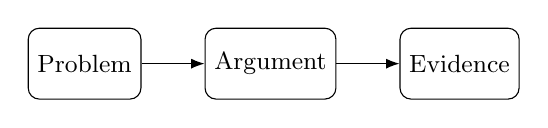
\begin{tikzpicture}[
  node distance=8mm,
  every node/.style={draw, rounded corners, minimum height=9mm, font=\small},
  >={Latex}
]
  \node (problem) {Problem};
  \node[right=of problem] (argument) {Argument};
  \node[right=of argument] (evidence) {Evidence};
  \draw[->] (problem) -- (argument);
  \draw[->] (argument) -- (evidence);
\end{tikzpicture}


  \medskip
  To do: Explain the main argument and its evidence, as recorded in the report.
\end{frame}

\begin{frame}{Limitations and next steps}
  To do: State what is established and what remains open.
\end{frame}

\begin{frame}{References}
  \bibliographystyle{plain}
  \bibliography{references}
\end{frame}

\end{document}
